\documentclass[12pt,a4paper]{article}
\usepackage[T1]{fontenc}
\usepackage{amsmath}
\usepackage{amssymb}
\usepackage{graphicx}
\usepackage[UTF8,heading=true]{ctex}
\usepackage{geometry}
\usepackage{diagbox}
\usepackage[]{float}
\usepackage{xeCJK}
\usepackage{indentfirst}
\usepackage{multirow}
\usepackage[section]{placeins}
\usepackage{caption}

\setCJKfamilyfont{zhsong}[AutoFakeBold = {5.6}]{STSong}
\newcommand*{\song}{\CJKfamily{zhsong}}

\geometry{a4paper,left=2cm,right=2cm,top=0.75cm,bottom=2.54cm}

\newcommand{\experiName}{微波干涉衍射实验}%实验名称
\newcommand{\supervisor}{易栖如}%指导教师
\newcommand{\name}{张钰堃}
\newcommand{\studentNum}{2022K8009926020}
\newcommand{\class}{2}%班级
\newcommand{\group}{08}%组
\newcommand{\seat}{11}%座位号
\newcommand{\dateYear}{2023}
\newcommand{\dateMonth}{11}%月
\newcommand{\dateDay}{14}%日
\newcommand{\room}{教学楼717}%地点
\newcommand{\others}{$\square$}

\ctexset{
    section={
        format+=\raggedright\song\large
    },
    subsection={
        name={\quad,.}
    },
    subsubsection={
        name={\qquad,.}
    }
}

\begin{document}
\noindent

\begin{center}

    \textbf{\song \zihao{-2} \ziju{0.5}《基础物理实验》实验报告}
    
\end{center}


\begin{center}
    \kaishu \zihao{5}
    \noindent \emph{实验名称}\underline{\makebox[28em][c]{\experiName}}
    \emph{指导教师}\underline{\makebox[9em][c]{\supervisor}}\\
    \emph{姓名}\underline{\makebox[6em][c]{\name}} 
    \emph{学号}\underline{\makebox[14em][c]{\studentNum}}
    \emph{分班分组及座号} \underline{\makebox[5em][c]{\class \ -\ \group \ -\ \seat }\emph{号}} (\emph{例}:\,1- 04- 5\emph{号})\\
    \emph{实验日期} \underline{\makebox[3em][c]{\dateYear}} \emph{年}
    \underline{\makebox[2em][c]{\dateMonth}}\emph{月}
    \underline{\makebox[2em][c]{\dateDay}}\emph{日}
    \emph{实验地点}\underline{{\makebox[4em][c]\room}}
    \emph{调课/补课} \underline{\makebox[3em][c]{否}}
    \emph{成绩评定} \underline{\hspace{8em}}
    {\noindent}
    \rule[5pt]{17.7cm}{0.2em}

\end{center}

\section{实验目的及要求}
    1.了解与学习微波产生的基本原理及传播和接受等基本特征\par
    2.观察微波衍射、干涉等实验现象\par
    3.观察模拟晶体的微波布拉格衍射现象\par
    4.通过迈克尔逊实验测量微波波长

\section{实验仪器}
    DHMS-1 型微波光学综合实验仪一套(图 1),包括:X 波段微波信号源、微波发生器、发
    射喇叭、接收喇叭、微波检波器、检波信号数字显示器、可旋转载物平台和支架,以及实验用附
    件(反射板、分束板、单缝板、双缝板、晶体模型、读数机构等)。
\section{实验原理}
    \subsection{微波双缝干涉}
    根据惠更斯原理,当一束波垂直入射到一块有两个狭缝的金属板上,两个狭缝就会称为次级波源,而且
    这两个波源发出的次级波是相干波。因此金属板后两束波满足波的干涉条件。当两个狭缝之间间隔为b,缝宽为a,
    且缝宽接近$\lambda $时,两束波在屏上叠加的波程差为
    \begin{equation}
        \Delta l = \left( {a + b} \right)\sin \varphi 
    \end{equation}

    当波程差为波长的整数倍时,干涉加强,所以干涉加强的角度为
    \begin{equation}
        \varphi  = \arcsin \left( {\frac{{k\lambda }}{{a + b}}} \right)\quad k = 1,2,3 \cdots 
    \end{equation}

    当波程差为波长的半整数倍时,干涉减弱,干涉减弱的角度为
    \begin{equation}
        \varphi  = \arcsin \left( {\frac{{2k - 1}}{2} \cdot \frac{\lambda }{{a + b}}} \right)\quad k = 1,2,3 \cdots 
    \end{equation}

    \subsection{微波单缝衍射}
    当微波入射到一宽度和微波波长相近的一狭缝时,微波在狭缝后会发生像光波一般的衍射现象。
    如果狭缝宽度为a,屏上某一点衍射的光强为
    \begin{equation}
        I \propto {\left\{ {\int_{ - \frac{a}{2}}^{\frac{a}{2}} {\exp \left( {\frac{{2\pi i}}{\lambda }x\sin \theta } \right)dx} } \right\}^2} \propto {\left( {\frac{{\sin \mu }}{\mu }} \right)^2}
    \end{equation}

    其中
    \begin{equation}
        \mu  = \frac{{\pi a\sin \varphi }}{\lambda }
    \end{equation}
    
    因此可以推出中央零级亮纹光强最强,中央两侧衍射波强度将迅速减小。除此之外,在一些点满足条件
    \begin{equation}
        a\sin \varphi  =  \pm k\lambda \quad k = 1,2,3 \cdots 
        \label{Yanshe:0}
    \end{equation}

    相应的衍射强度为0。测得第一衍射最小值所对应的角度,利用公式(\ref{Yanshe:0}),可以求出微波波长

    \subsection{微波迈克尔逊干涉}
    \begin{figure}[H]
        \centering
        \includegraphics[scale=3.0]{迈克尔逊干涉.png}
        \caption{迈克尔逊干涉原理}
    \end{figure}
    迈克尔逊干涉装置如图所示。发射喇叭发出的微波在半透板处被分为两束波,分别向反射板A,B方向传播,两束反射光
    在接收喇叭处发生干涉。因此,两束波的相位差为$ \pm 2k\pi \quad k = 1,2,3 \cdots $时,干涉
    加强,相位差为$ \pm \left( {2k - 1} \right)\pi \quad k = 1,2,3 \cdots $时,干涉减弱。
    
    因此,当A,B两板其中一块固定,另一块前后移动时,接受信号从一个极值到另一个极值,则反射板
    移动了$\frac{\lambda }{2}$的距离,我们可以根据距离算出波长。

    \subsection{微波布拉格衍射}
    \subsubsection{晶体的结构}
        \begin{figure}[H]
            \centering
            \includegraphics[scale=1.5]{晶体.png}
            \includegraphics[scale=1.3]{晶面.png}
            \caption{晶体的结构}
        \end{figure}
    组成晶体的原子或分子按照一定规律在空间中周期性排列,其中最简单的是按照固定距离a在空间中按顺序重复排列,
    形成简单的立方点阵,原子间距a称为晶格常数。组成晶体的原子可以看做分别处于一系列相互平行
    且间距固定的平面上,这些平面被称为晶面。图中展示了三种晶面的取法。

    \subsubsection{布拉格衍射}
    二维光栅的衍射实际上是平面上的小孔衍射波相干叠加的结果。在晶体的衍射中,三维空间中原子
    组成的格点可以看做二维光栅中的小孔,晶体对波的衍射是每个格点上原子产生散射波的相干叠加。
    布拉格衍射可以看做是有两个过程,第一个过程是同一晶面上个原子发出的散射波的相干叠加,第二个
    过程是不同晶面之间衍射波的相干叠加。

    同一晶面上的原子发出的的散射波遵从反射定律,这些波波程差为0。不同波之间波程差在第二个过程中
    产生。根据干涉的知识,在满足
    \begin{equation}
        2d\sin \theta  = k\lambda \quad k = 1,2,3 \cdots 
    \end{equation}
    时,会形成干涉极大。从实验中可以测量衍射极大角,根据波长,可以求出晶面间距d,进一步可以求出晶格
    常数a。
\section{实验内容}
    \subsection{实验准备}
    1.调节实验仪器四只脚使底盘水平\par
    2.调节反射喇叭、接收喇叭、接受臂、活动臂为直线对齐状态,调节接收、发射喇叭高度相同\par
    3.连接X波段微波信号源,调节微波发生器频率和功率
    \subsection{微波双缝干涉}
    1.调节双缝干涉板的缝宽\par
    2.将双缝干涉板安置在支座上,调节角度使双缝板平面与载物台上的$90^{\circ}$指示线一致。
    转动平台使固定臂的指针在$180^{\circ}$处。\par
    3.调节信号使显示器示数较大,然后在$0^{\circ}$线的两侧,每隔$2^{\circ}$读取一次液晶显示器
    的读数,记录读数。\par
    4.根据所得数据,确定一级极大、零级极小、一级极小角度所在大致区间,在这些区间里每隔$1^{\circ}$记录一次数据,找出
    一级极大、零级极小、一级极小的角度\par

    \subsection{微波迈克尔逊干涉}
    1.在微波前进方向放置一块玻璃板,使玻璃板平面与$45^{\circ}$线在同一平面上\par
    2.调节固定臂指针指向$90^{\circ}$刻度线,接收臂指针指向$0^{\circ}$刻度线,根据迈克尔逊干涉仪原理
    安置固定反射板、可移动反射板、接收喇叭。\par
    3.旋转读数机构上的手柄,记录四个干涉最小点的刻度。
    \subsection{微波布拉格衍射}
    1.将模拟晶体架插在载物平台的四颗螺柱上,使(100)发现正对平台上的$0^{\circ}$刻度线\par
    2.顺时针转动载物台$30^{\circ}$,然后把接收臂顺时针转到$30^{\circ}$处\par
    3.转动载物台和接收臂,入射角和出射角每隔$2^{\circ}$记录一次数据\par
    4.根据所得数据,确定衍射极大角度大致范围,在这个范围内每隔$1^{\circ}$记录一次数据\par
    5.改用(110)晶面,重复1-4操作
    \subsection{微波单缝衍射}
    1.调整单缝衍射板缝宽,将单缝衍射板置于载物台上\par
    2.转动载物台,使单缝衍射板$180^{\circ}$刻度线与发射臂的指针一致,转动接收臂使其指针指向载物台的$0^{\circ}$刻度线\par
    3.转动接收臂,每隔$2^{\circ}$记录一次接收信号的大小\par
    4.根据所得数据,确定一级极小大致范围,在这个范围内每隔$1^{\circ}$记录一次数据\par

    \section{实验数据与数据处理}
    \subsection{实验前条件确认}
    实验条件确认:微波频率9.4GHz\quad 微波波长3.1915cm
    \begin{table}[H]
        \centering
        \caption{微波实验仪对准确认}
        \begin{tabular}{|l|l|l|l|}
        \hline
            角度($^{\circ}$) & 0 & 20 & -20 \\ \hline
            电压(mV) & 93 & 6.3 & 6.4 \\ \hline
        \end{tabular}
    \end{table}
    由数据可知仪器基本已对准
    \subsection{双缝干涉实验}
    \begin{table}[H]
        \centering
        \caption{双缝干涉实验数据}
        \begin{tabular}{|l|l|l|l|l|l|l|l|l|l|}
        \hline
            $\theta(^\circ)$ & 0 & 2 & 4 & 6 & 8 & 10 & 12 & 14 & 16 \\ \hline
            $U_{\theta+}(mV)$ & 93 & 95 & 83 & 63 & 34 & 4.8 & 0 & 0.1 & 3.6 \\ \hline
            $U_{\theta-}(mV)$ & 93 & 65 & 27 & 4 & 0.9 & 3 & 9 & 23 & 51 \\ \hline
            $\theta(^\circ)$ & 18 & 20 & 22 & 24 & 26 & 28 & 30 & 32 & 34 \\ \hline
            $U_{\theta+}(mV)$ & 16 & 36 & 49 & 55 & 50 & 27 & 5 & 0.6 & 0.4 \\ \hline
            $U_{\theta-}(mV)$ & 70 & 84 & 59 & 30.5 & 5 & 2.3 & 2.5 & 2.7 & 8.8 \\ \hline
            $\theta(^\circ)$ & 36 & 38 & 40 & 42 & 44 & 46 & 48 & 50 & ~ \\ \hline
            $U_{\theta+}(mV)$ & 1 & 1.4 & 4.5 & & &&&&\\ \hline
            $U_{\theta-}(mV)$ & 13.5 & 5 & 0.1 &  &&&&& \\ \hline
        \end{tabular}
    \end{table}
    \begin{figure}[H]
        \caption{双缝干涉实验数据图像}
        \centering
        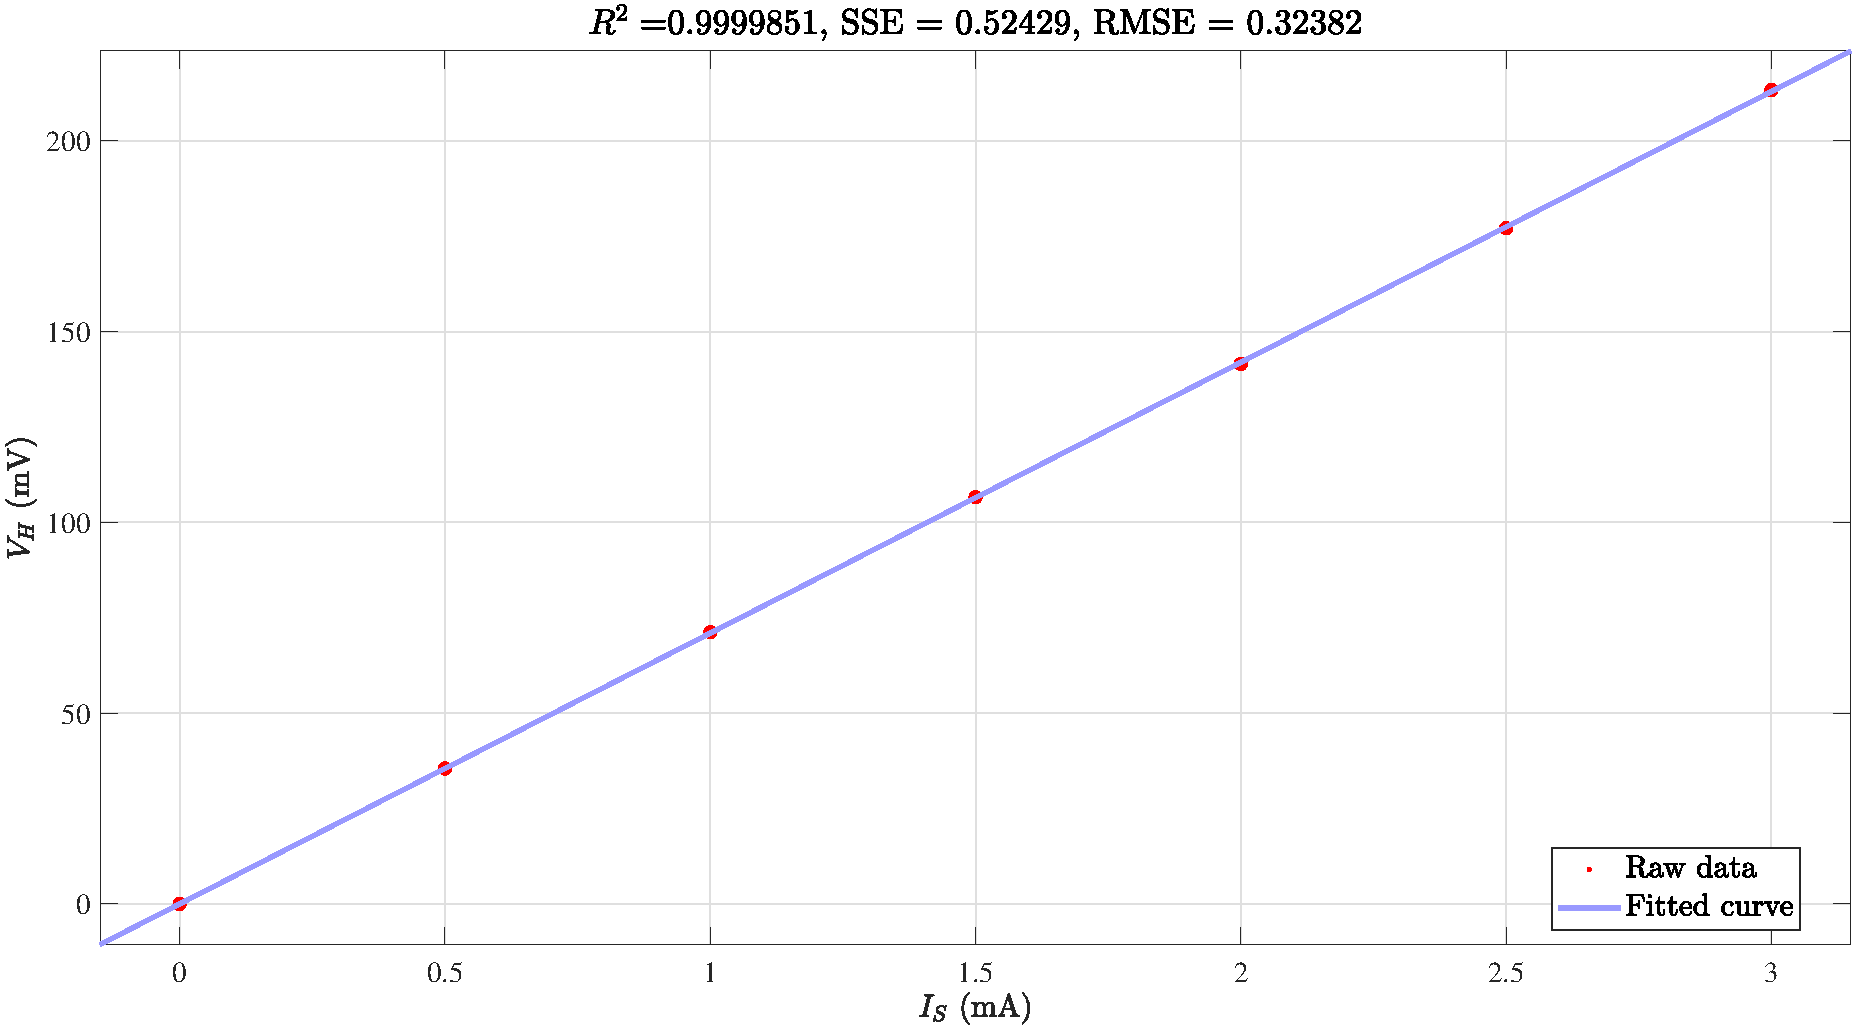
\includegraphics[scale=0.25,angle=180]{1.jpg}
    \end{figure}
    \begin{table}[H]
        \centering
        \caption{一级极大附近扫描数据}
        \begin{tabular}{|l|l|l|l|l|l|l|l|l|}
        \hline
            $\theta(^\circ)$ & 19 & 20 & 21 & 22 & 23 & 24 & 25  \\ \hline
            $U_{\theta+}(mV)$ & 34 & 39 & 42 & 50 & 55 & 55 & 50 \\ \hline
            $\theta(^\circ)$ & 19 & 20 & 21 & 22 & 23 & 24 & 25  \\ \hline
            $U_{\theta-}(mV)$ & 80 & 74 & 90 & 70 & 64 & 45 & 20  \\ \hline
        \end{tabular}
    \end{table}

    可以看出图像对称性良好,而且在角度接近0时干涉极大,符合理论预言。粗略估计,一级极大在$22^{\circ}$附近;
    零级极小在$10^{\circ}$附近;一级极小在$33^{\circ}$附近。接下来在这几个角度附近进行精细扫描。

    数据与理论值出现了一定误差。比如实验测得的零级极大并不严格在角度为0处,以及图像没有严格对称。可能的误差原因包括:
    
    读数时仪器无法给出确定的数值,示数一直在小幅波动,需要凭借主观判断确定一个大概的平均值,因而造成读数误差。

    实验前校准时实验仪器没有严格对正,造成零点由有偏移。
    \begin{figure}[H]
        \centering
        \caption{一级极大扫描数据图像}
        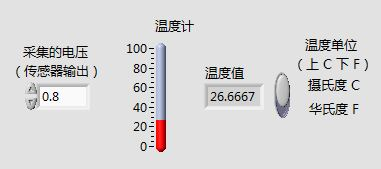
\includegraphics[scale=0.25,angle=180]{2.jpg}
    \end{figure}

    \begin{figure}[H]
        \centering
        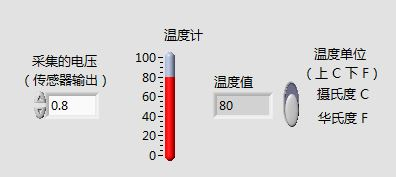
\includegraphics[scale=0.25,angle=180]{3.jpg}
    \end{figure}

    由两图峰值对应的角度绝对值求平均值,可以消去角度零点的偏移,一级极大对应的角度$\theta_0=22.3^{\circ}$。
    代入公式求出微波波长,得到$\lambda {\rm{ = }}\left( {a + b} \right)\sin {\theta _0} = 3.18cm$。相对
    误差为$0.31\%$,与实际微波波长符合的很好。

    \begin{table}[H]
        \centering
        \caption{零级极小附近扫描数据}
        \begin{tabular}{|l|l|l|l|l|l|l|l|l|}
        \hline
            $\theta(^\circ)$ & 7 & 8 & 9 & 10 & 11 & 12 & 13  \\ \hline
            $U_{\theta+}(mV)$ & 27 & 34 & 5 & 4.8 & 0.5 & 0 & 0.4 \\ \hline
            $\theta(^\circ)$ & 7 & 8 & 9 & 10 & 11 & 12 & 13 \\ \hline
            $U_{\theta-}(mV)$ & 9 & 0.9 & 3 & 3 & 7 & 9 & 15  \\ \hline
        \end{tabular}
    \end{table}

    \begin{figure}[H]
        \centering
        \caption{零级极小扫描数据图像}
        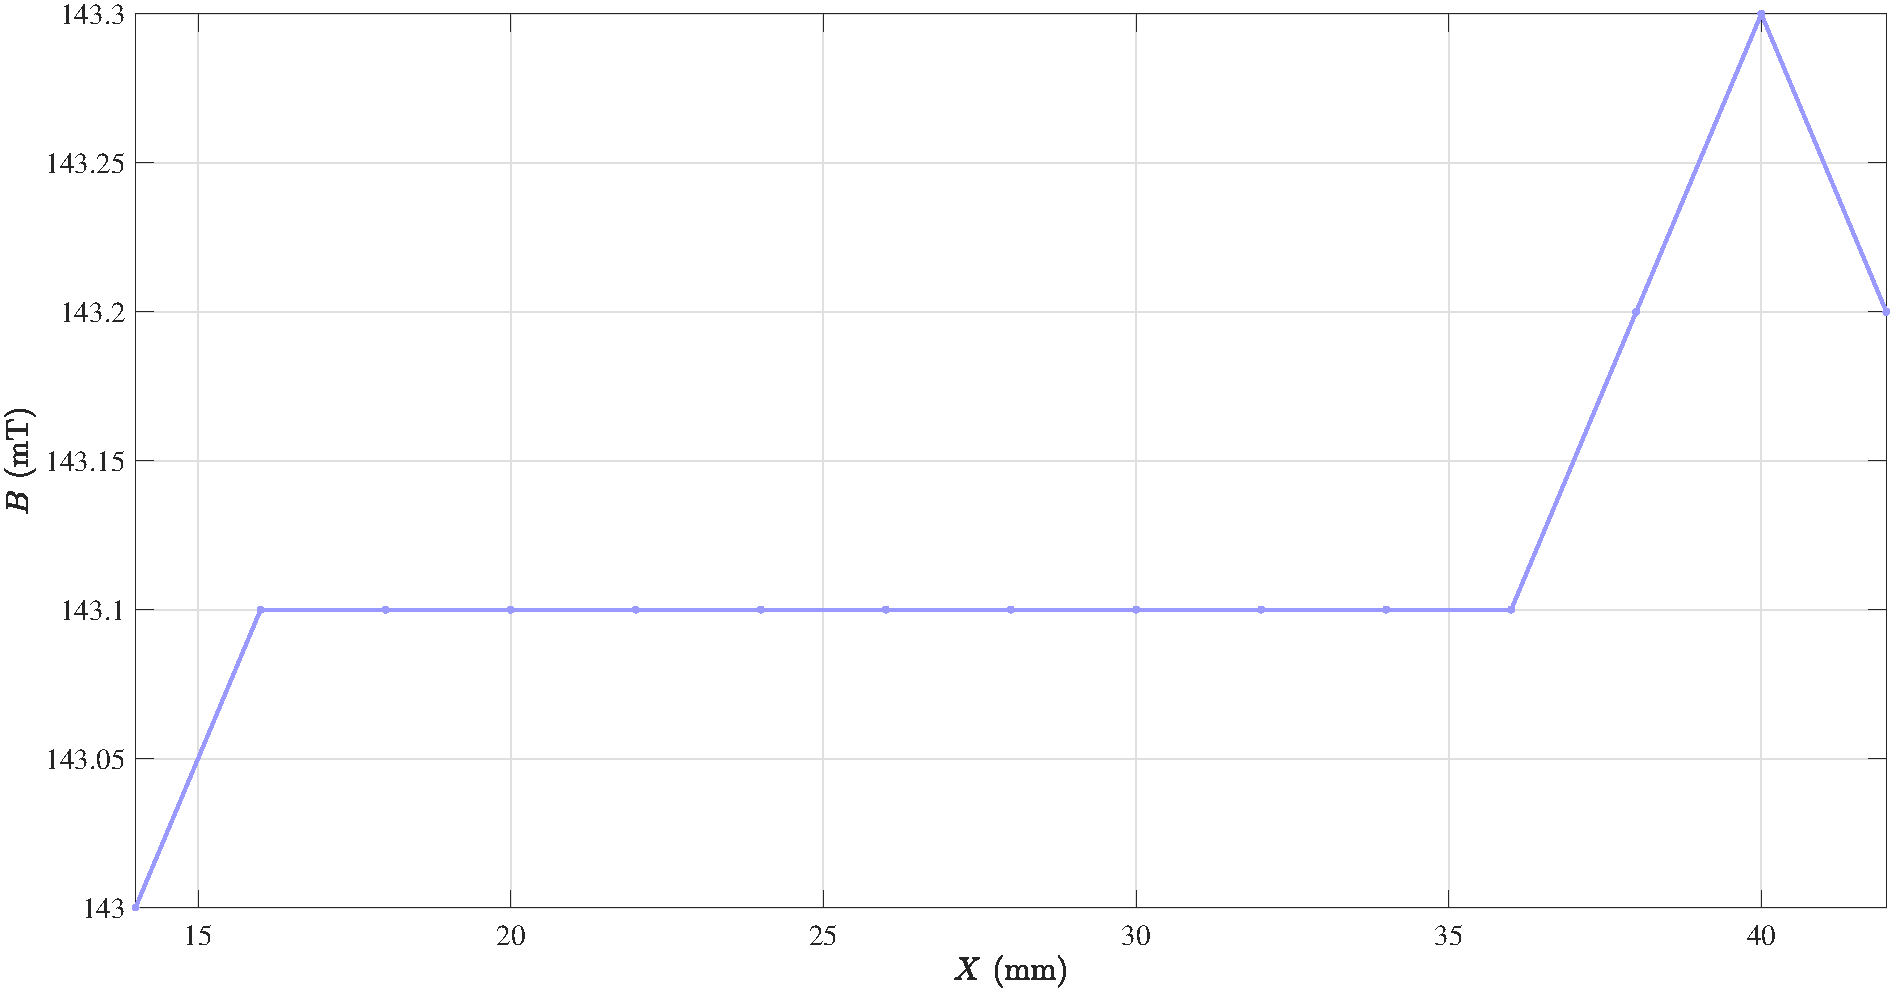
\includegraphics[scale=0.25,angle=180]{4.jpg}
    \end{figure}
    \begin{figure}[H]
        \centering
        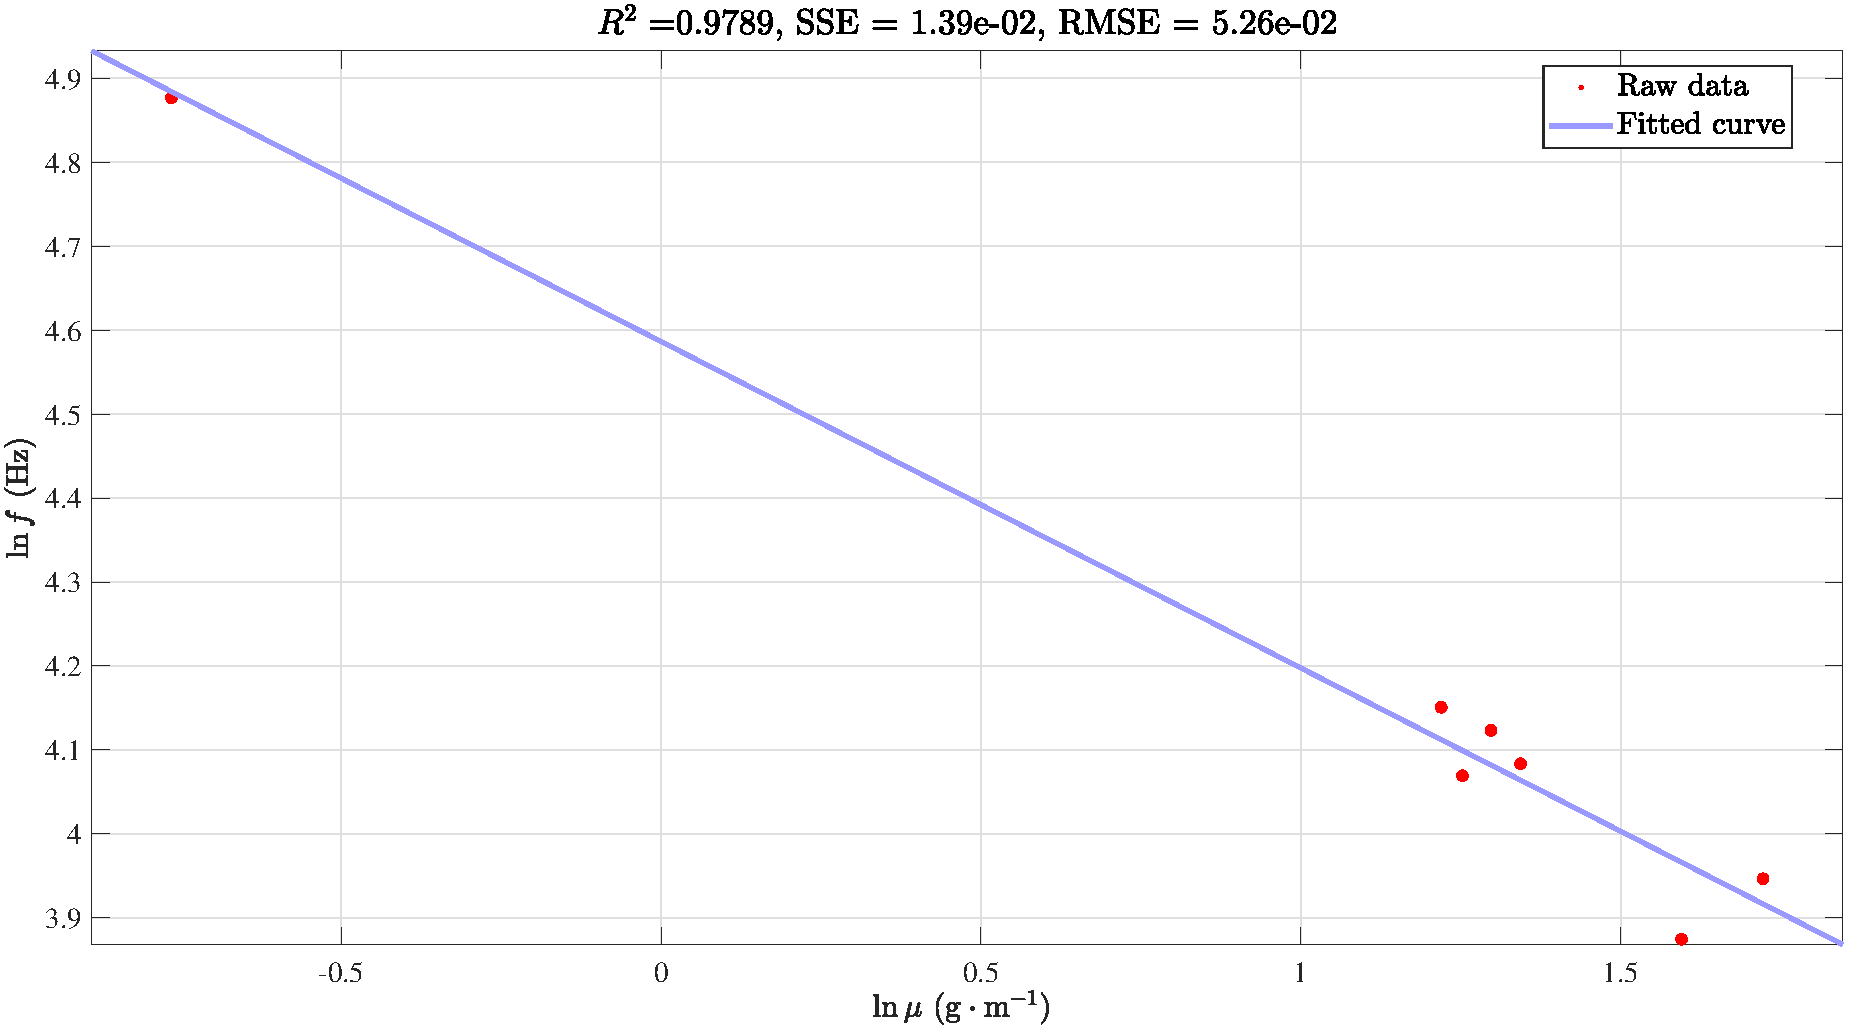
\includegraphics[scale=0.25,angle=180]{5.jpg}
    \end{figure}

    由两图峰值对应的角度绝对值求平均值,可以消去角度零点的偏移,零级极小对应的角度$\theta_0=10^{\circ}$。
    代入公式可以求出微波波长,得到$\lambda  = 2\left( {a + b} \right)\sin {\theta _0} = 3.05cm$,
    相对误差$4.43\%$,与理论值接近,但是误差相对较大。

    \begin{table}[H]
        \centering
        \caption{一级极小附近扫描数据}
        \begin{tabular}{|l|l|l|l|l|l|l|l|l|1|}
        \hline
            $\theta(^\circ)$ & 26 & 27& 28 & 29 & 30 & 31& 32 & 33&34 \\ \hline
            $U_{\theta+}(mV)$ & 50& 35 & 27 & 9.5 & 3 & 1 & 0.6 & 0.2&0.4 \\ \hline
            $\theta(^\circ)$ & 26 & 27& 28 & 29 & 30 & 31& 32 & 33&34 \\ \hline
            $U_{\theta-}(mV)$ & 5 & 2.5 & 2.3 & 2.5 & 2.5 & &2.7 & &8.8 \\ \hline
        \end{tabular}
    \end{table}

    \begin{figure}[H]
        \centering
        \caption{一级极小扫描数据图像}
        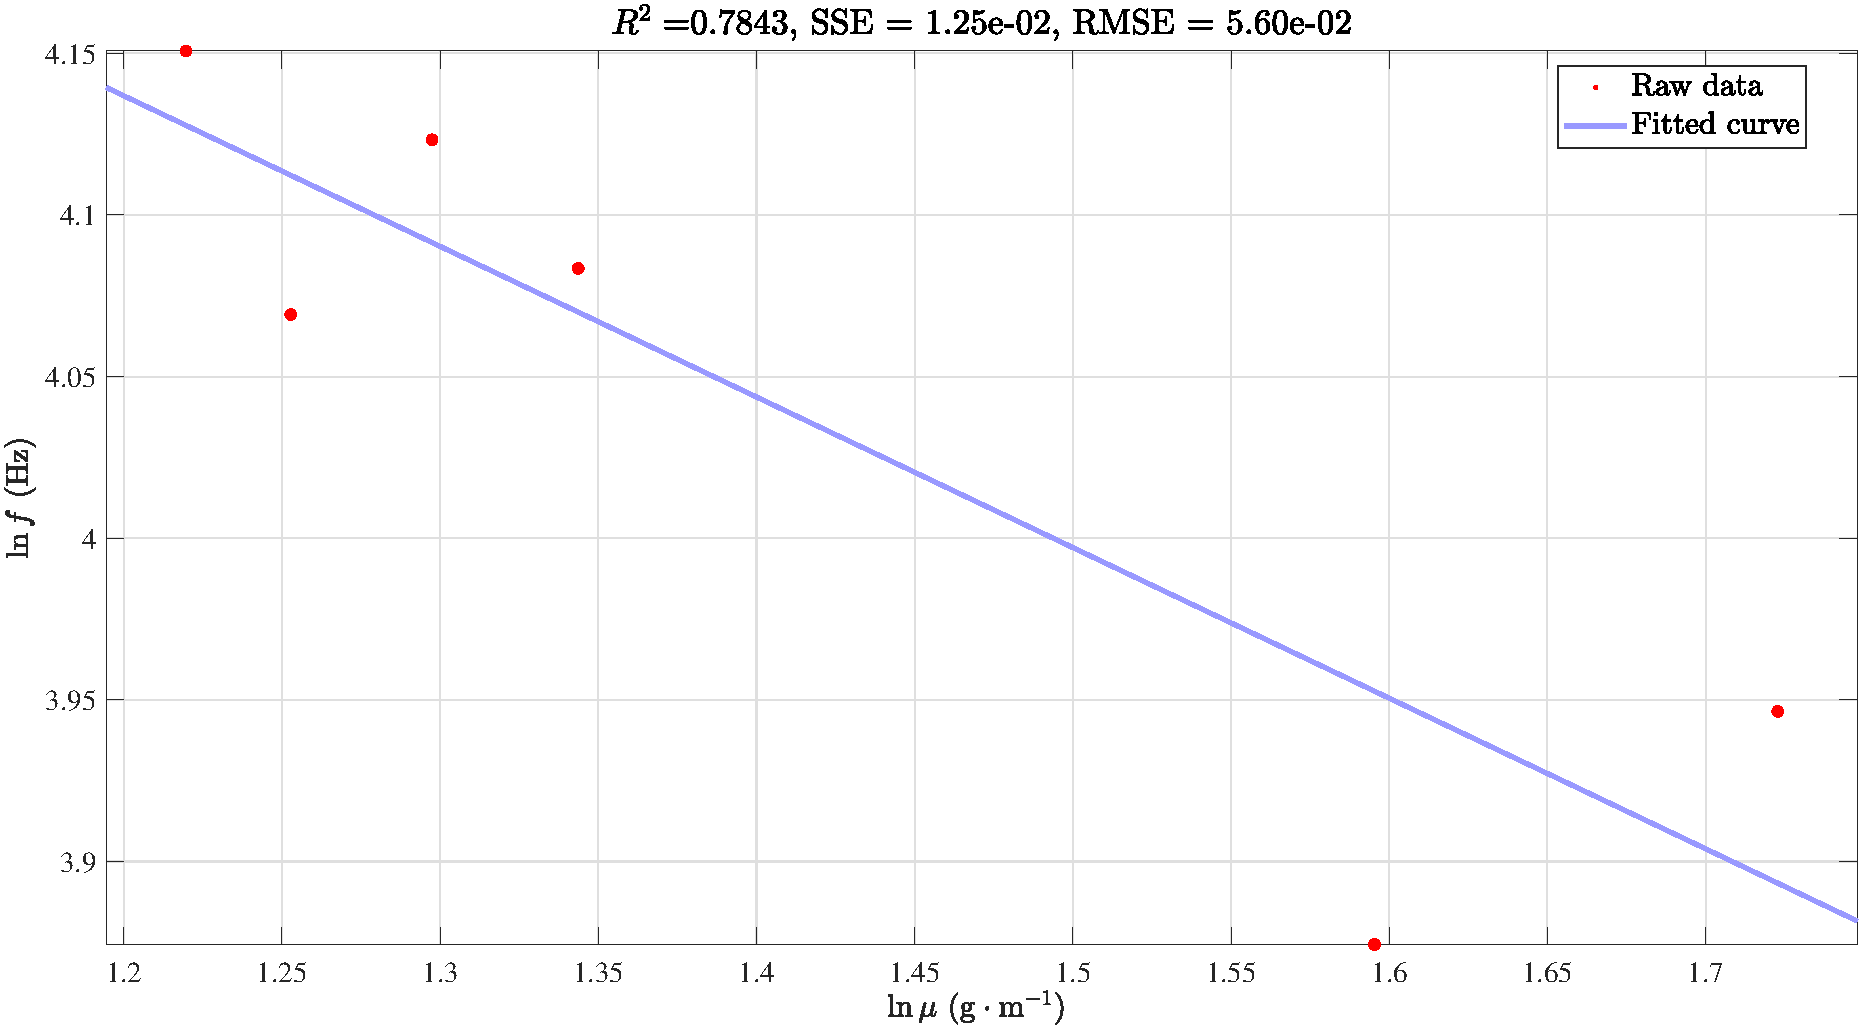
\includegraphics[scale=0.25,angle=180]{6.jpg}
    \end{figure}

    \begin{figure}[H]
        \centering
        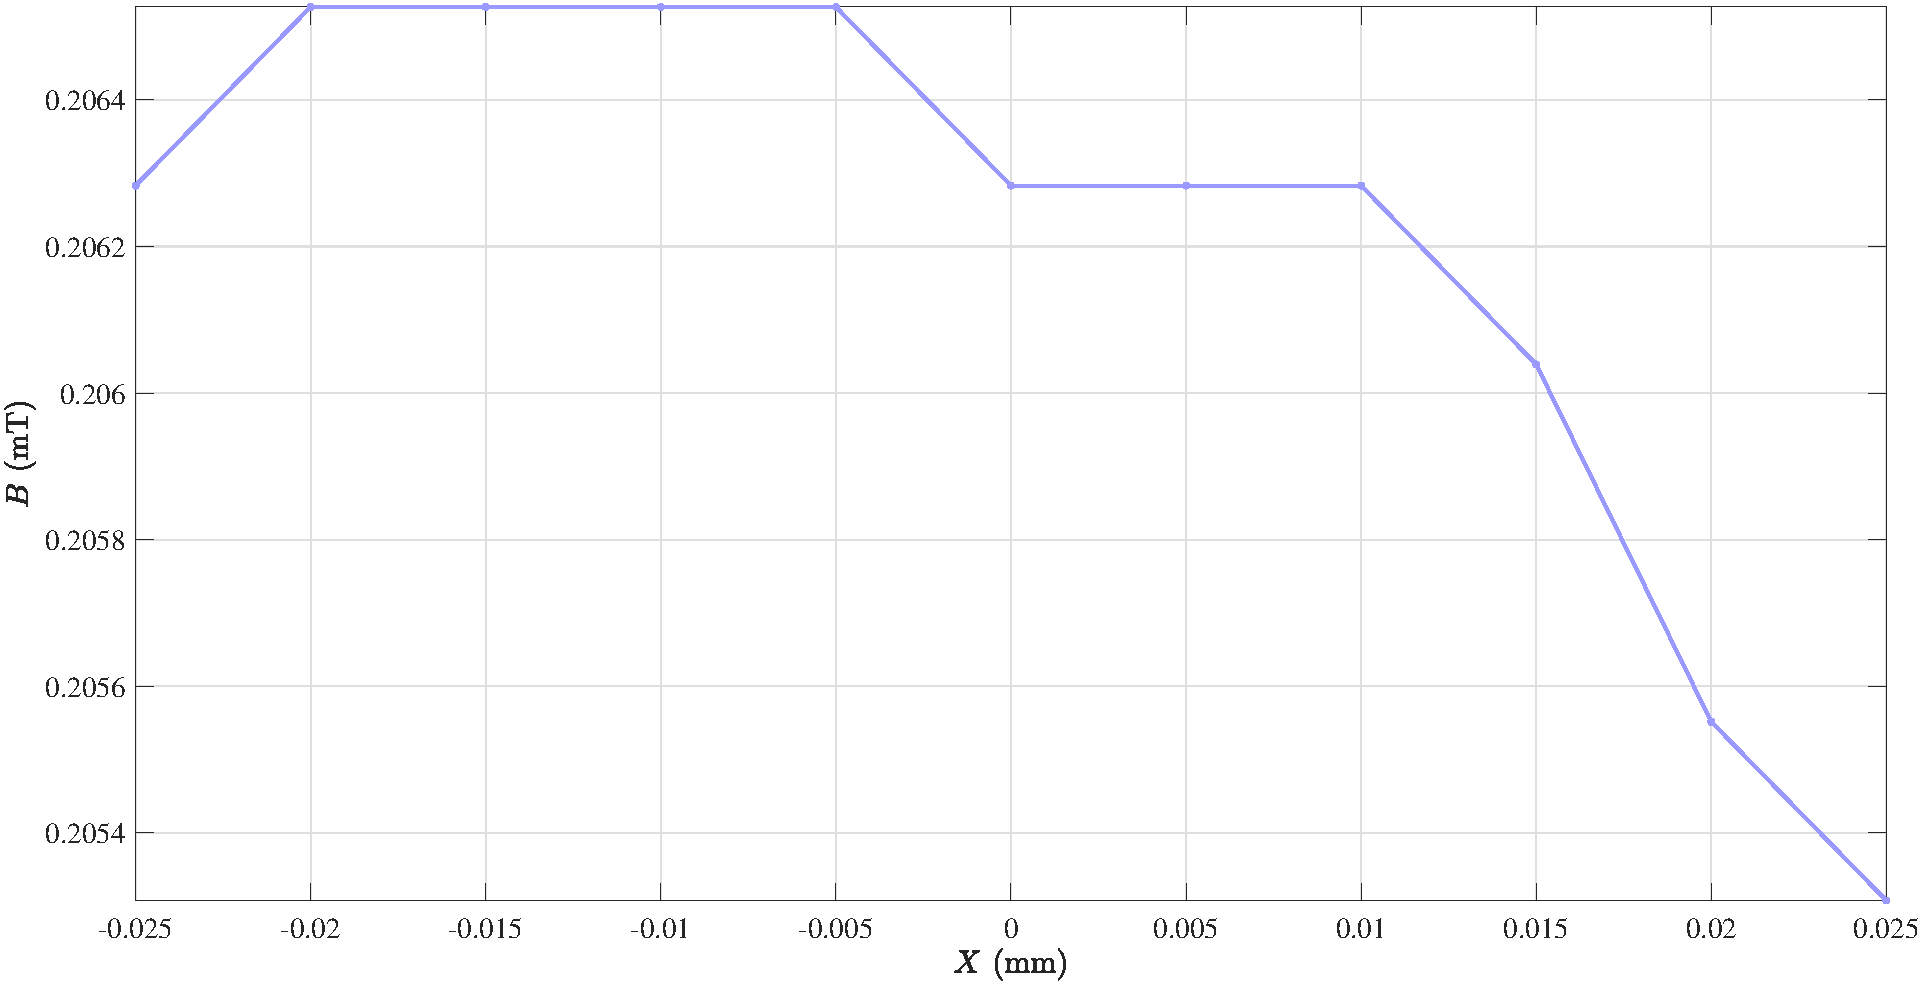
\includegraphics[scale=0.25,angle=180]{8.jpg}
    \end{figure}

    由两图极小值对应角度的绝对值求出平均值可以消去零点的偏移,一级极小对应的角度为${\theta _0}{\rm{ = }}30.5^\circ $,
    代入公式求出微波波长$\lambda {\rm{ = }}\frac{2}{3}\left( {a + b} \right)\sin {\theta _0} = 2.87cm$,
    相对误差$10.0\% $,与理论值有较大误差。

    可能的误差原因有:

    在角度值为正时,一级极小附近连续多个角度显示的的电压值几乎为零,这导致很难判断一级极小的具体位置。
\subsection{微波迈克尔逊干涉实验}
   
    \begin{table}[H]
        \centering
        \caption{迈克尔逊干涉仪实验数据}
        \begin{tabular}{|l|l|l|l|l|}
        \hline
            最小点读数(mm) & 65.0 & 50.0 & 36.0& 21.0 \\ \hline
        \end{tabular}
    \end{table}

    用逐差法处理数据,得到$\Delta L = 15.0mm,\lambda  = 2\Delta L = 3.0cm$,相对误差
    为$9.4{\rm{\% }}$,与理论值有较大误差。\par
    可能的误差原因有:\par
    示数精度不足,仪器没有完全对正。

\subsection{微波布拉格衍射实验}
    \begin{table}[H]
        \centering
        \caption{实验仪器对准确认}
        \begin{tabular}{|l|l|l|l|}
        \hline
            角度$(^{\circ})$ & 0 & 20 & -20 \\ \hline
            电压(mV) & 159.1 & 13.9 & 13.8 \\ \hline
        \end{tabular}
    \end{table}

    \subsubsection{100晶面布拉格衍射}
        \begin{table}[H]
            \centering
            \caption{100晶面布拉格衍射实验数据}
            \raggedright{$\qquad\qquad\quad$晶面间距$4cm$\par}
            \centering
            \begin{tabular}{|l|l|l|l|l|l|l|l|l|l|}
            \hline
                $\varphi_1(^\circ)$ & 30 & 32 & 34 & 36 & 38 & 40 & 42 & 44 & 46 \\ \hline
                U(mV) & 2.9 & 4.5 & 3.7 & 3.7 & 4.9 & 9.5 & 13.3 & 5.3 & 0.7 \\ \hline
                $\varphi_1(^\circ)$ & 48 & 50 & 52 & 54 & 56 & 58 & 60 & 62 & 64 \\ \hline
                U(mV) & 1.7 & 9.8 & 11.3 & 1.3 & 1.8 & 3 & 2.4 & 26.7 & 40 \\ \hline
                $\varphi_1(^\circ)$ & 66 & 68 & 70 & 72 & 74 & 76 & 78 & 80 & ~ \\ \hline
                U(mV) & 43 & 121& 147 & 27.2 & 2.9& 21.5 & 12.6 & 0.2 & ~ \\ \hline
            \end{tabular}
        \end{table}
\begin{figure}
    \centering
    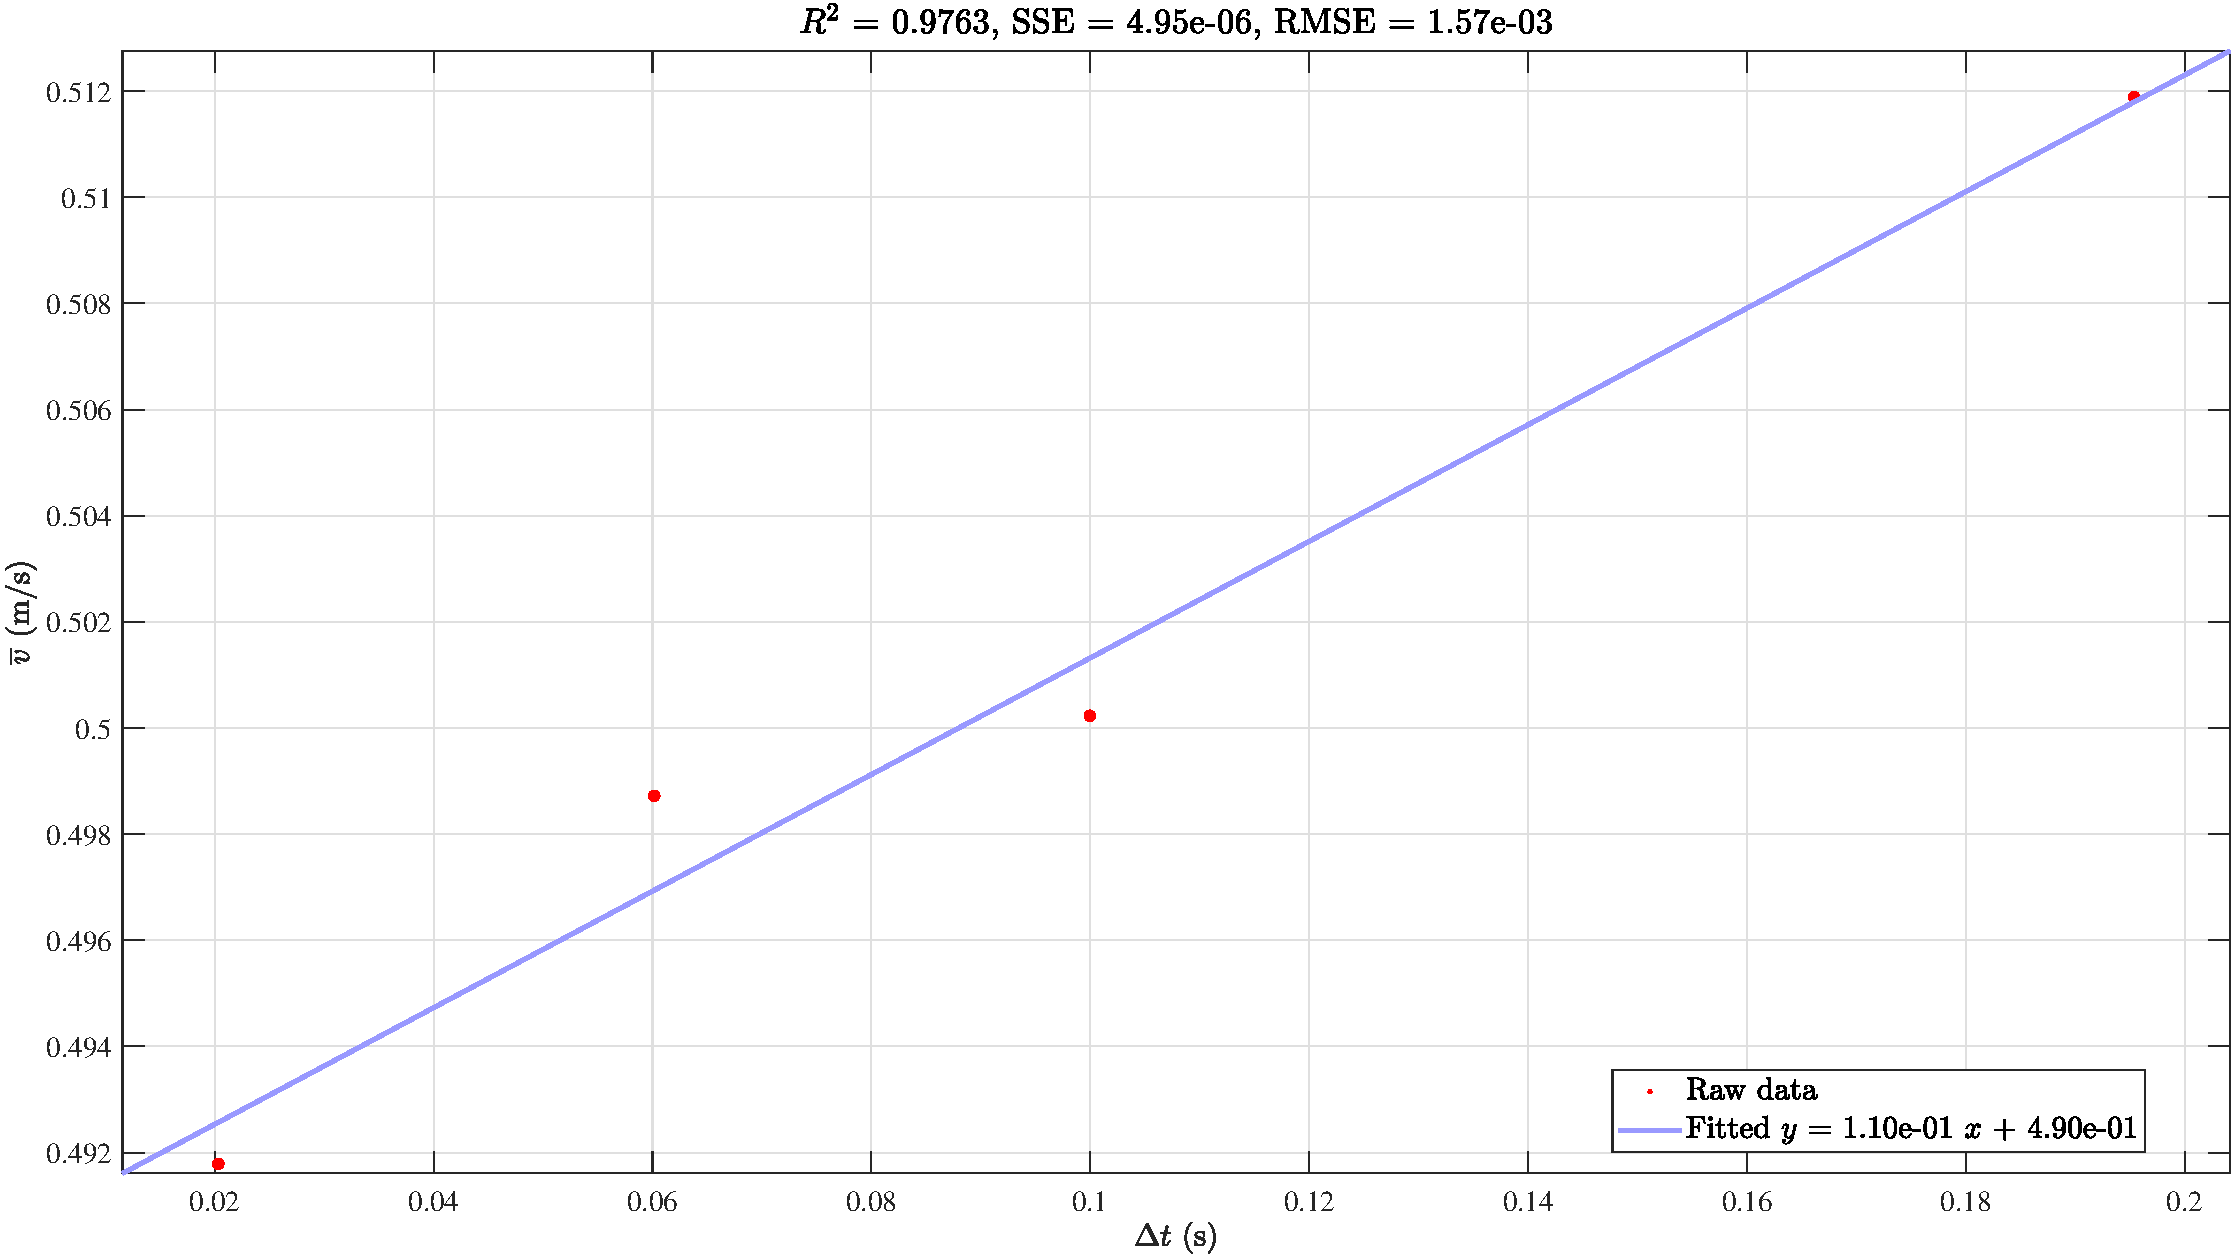
\includegraphics[scale=0.25,angle=180]{9.jpg}
\end{figure}
        从图像中可以发现,衍射极大值在$70^{\circ}$时出现,在$70^{\circ}$附近精细扫描

        \begin{table}[H]
            \centering
            \caption{衍射极大角度附近扫描数据}
            \begin{tabular}{|l|l|l|l|l|l|l|l|l|l|}
            \hline
                $\varphi_1(^\circ)$ & 68 & 69 & 70 & 71 & 72 \\ \hline
                U(mV) & 121 & 136 & 147 & 124 & 27.2 \\ \hline
            \end{tabular}
        \end{table}

        \begin{figure}[H]
            \centering
            \caption{100晶面布拉格衍射实验数据图像}
            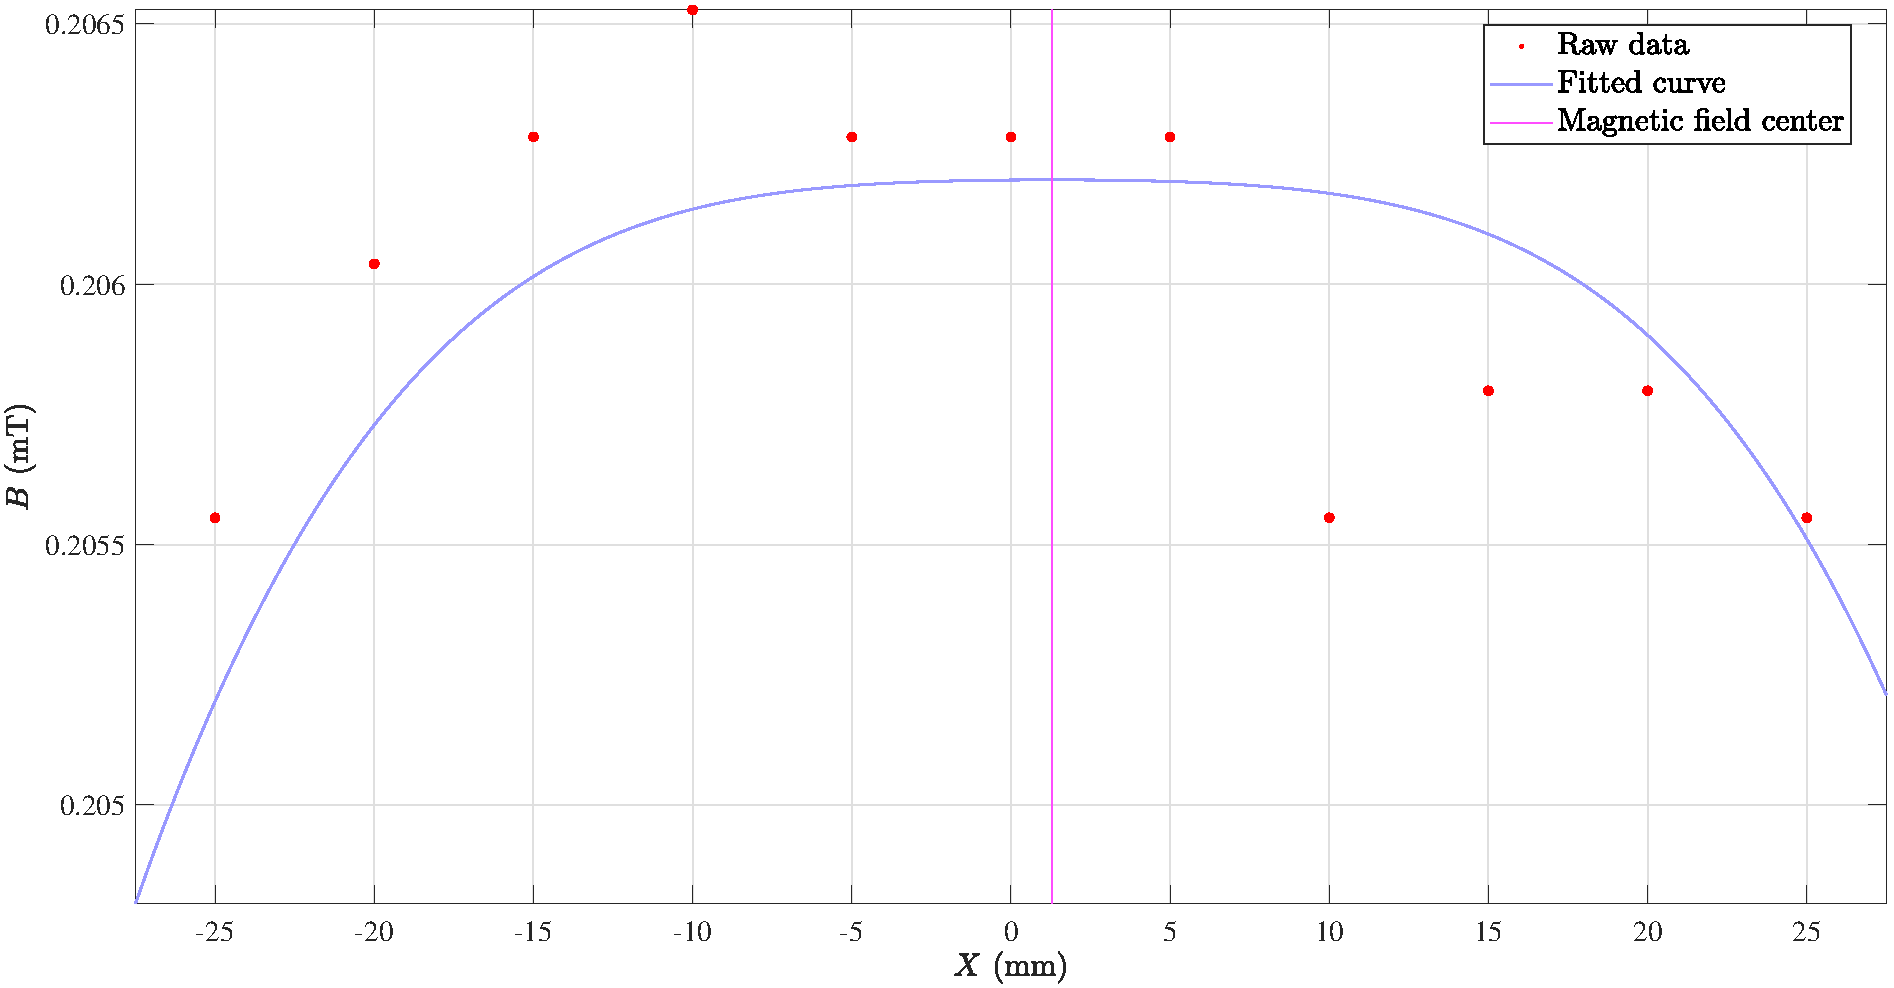
\includegraphics[scale=0.25]{7.jpg}
        \end{figure}

        根据数据可以发现,衍射极大值在$70^{\circ}$,代入公式得到波长$\lambda {\rm{ = 2dcos}}\beta {\rm{ = 3}}{\rm{.04cm}}$,
        相对误差为$4.7\%$,与理论值相近但有一定误差。
    
    \subsubsection{110晶面布拉格衍射}   
    \begin{table}[H]
        \centering
        \caption{110晶面布拉格衍射实验数据}
        \raggedright{$\qquad\qquad\qquad\quad$晶面间距$4cm$\par}
        \centering
        \begin{tabular}{|l|l|l|l|l|l|l|l|l|l|}
        \hline
            $\varphi_1(^\circ)$ & 30 & 32 & 34 & 36 & 38 & 40 & 42 & 44 & 46 \\ \hline
            U(mV) & 0 & 0 & 0& 0 & 0 & 0 & 0.1 & 0.1 & 0.1 \\ \hline
            $\varphi_1(^\circ)$ & 48 & 50 & 52 & 54 & 56 & 58 & 60 & 62 & 64 \\ \hline
            U(mV) & 0.3 & 0.3 & 1 & 3.6 & 7.7 & 11.5 & 14.3 & 3.5 & 1.6 \\ \hline
            $\varphi_1(^\circ)$ & 66 & 68 & 70 & ~ & ~ & ~ & ~ & ~ & ~ \\ \hline
            U(mV) & 0.4 & 0 & 0 & ~ & ~ & ~ & ~ & ~ & ~ \\ \hline
        \end{tabular}
    \end{table}
\begin{figure}
    \centering
    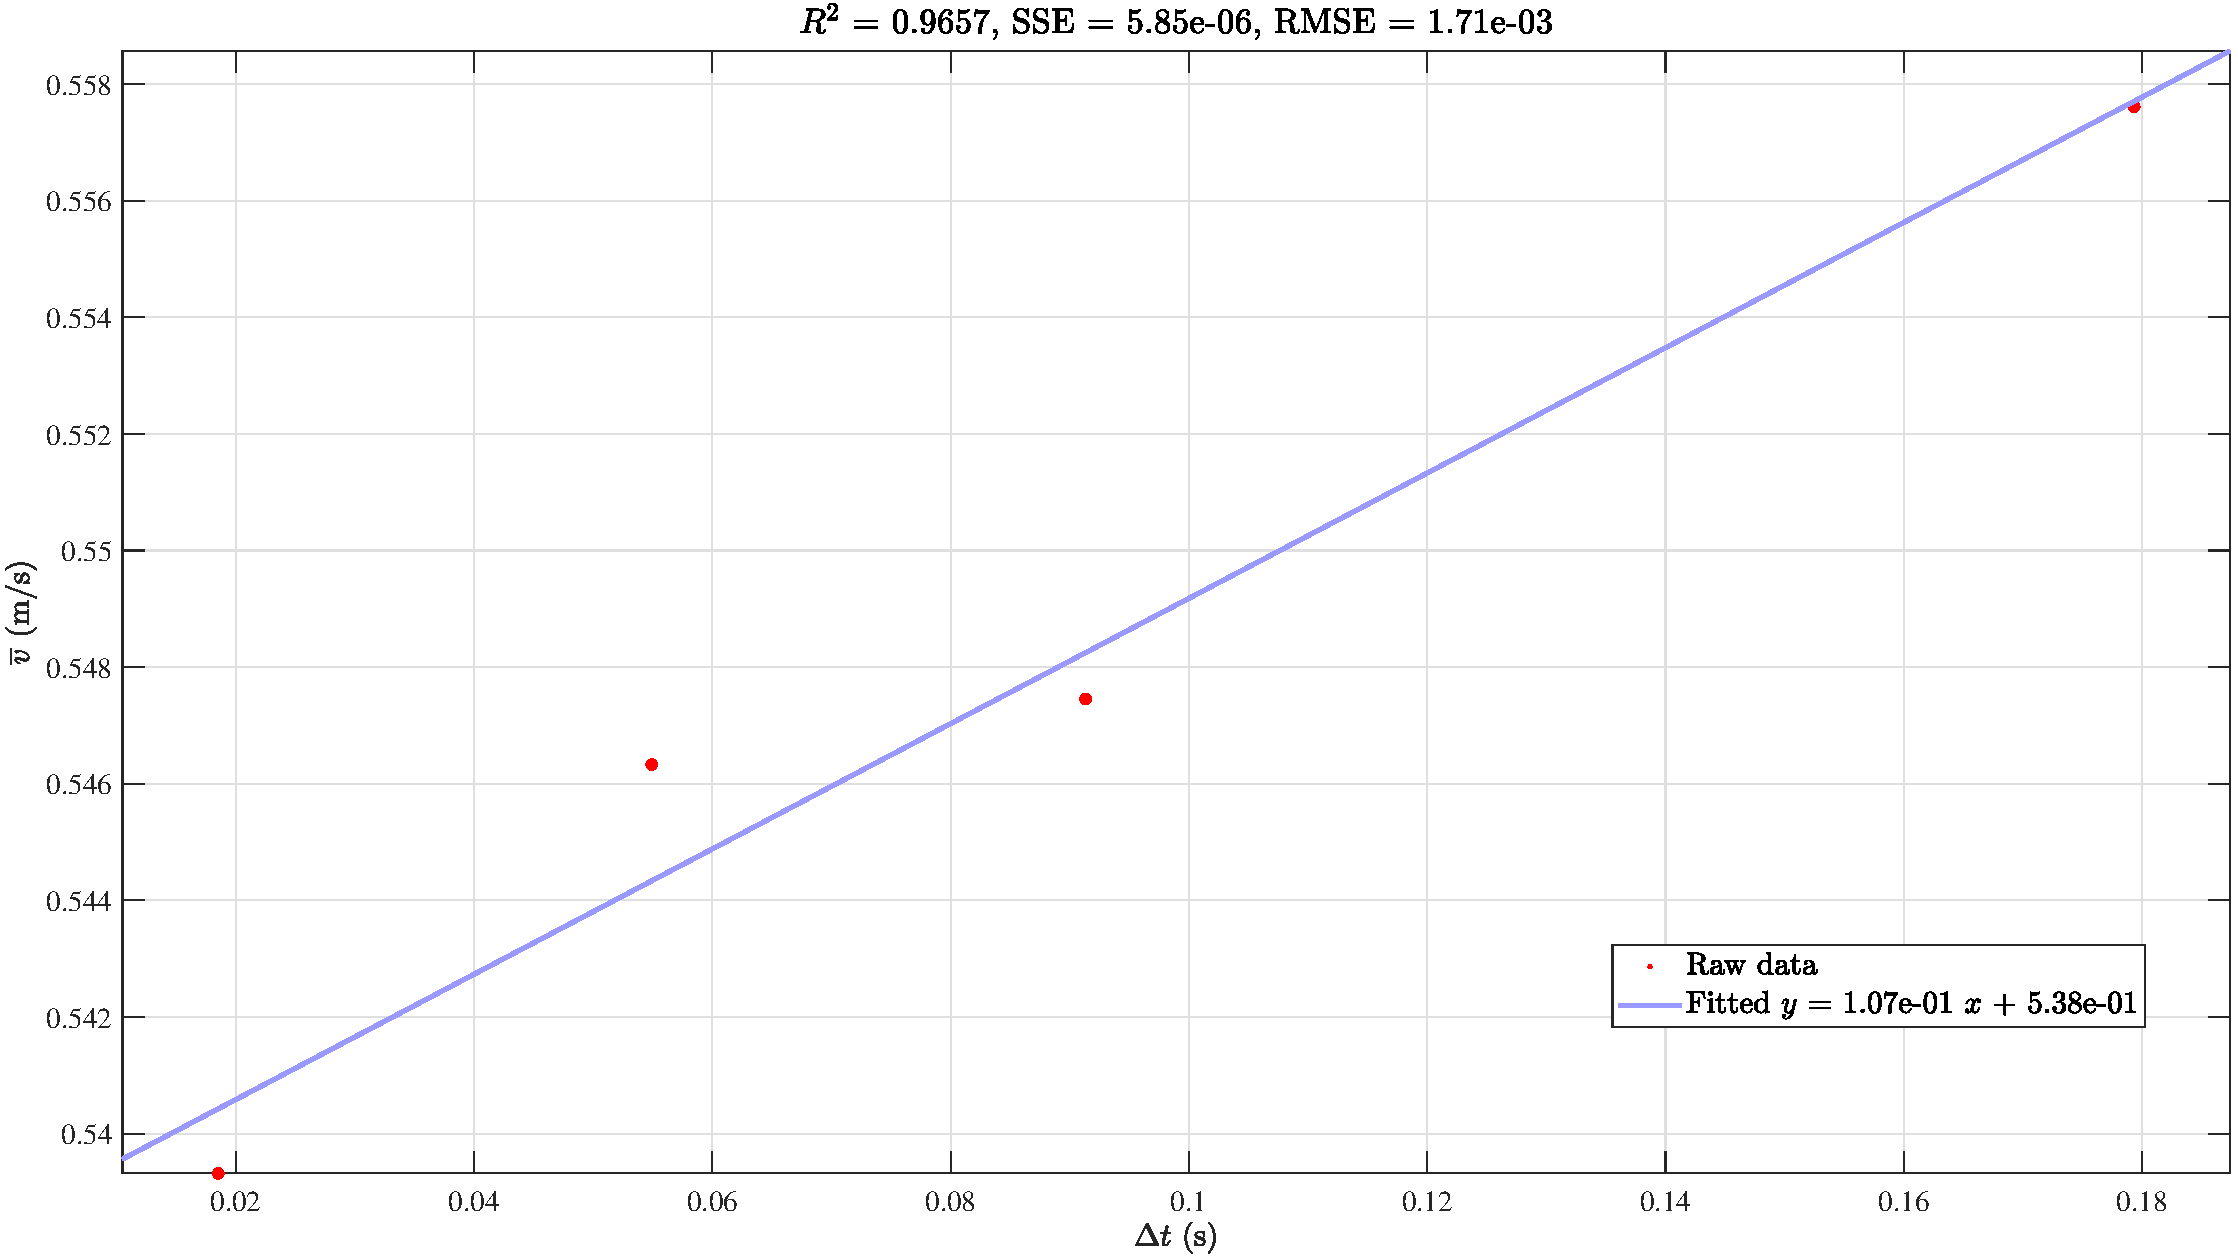
\includegraphics[scale=0.25,angle=180]{10.jpg}
\end{figure}
    根据数据可以发现,衍射极大值在$60^{\circ}$,在$60^{\circ}$附近进行精细扫描

    \begin{table}[H]
        \centering
        \caption{衍射极大角度附近扫描数据}
        \begin{tabular}{|l|l|l|l|l|l|l|l|l|l|}
        \hline
            $\varphi_1(^\circ)$ & 58& 59 & 60& 61 & 62 \\ \hline
            U(mV) & 11.5 &14.9 & 14.3 & 13 & 3.5 \\ \hline
        \end{tabular}
    \end{table}

    \begin{figure}[H]
        \centering
        \caption{110晶面布拉格衍射实验数据图像}
        \includegraphics[scale=0.25,angle=180]{11.jpg}
    \end{figure}

    观察图像可知,衍射最大在$59^{\circ}$,代入公式计算波长,得到$\lambda  = 2d\cos \beta  = 2.84cm$,
    相对误差为$11.0\%$,与理论值有较大误差。\par
    可能的误差原因有:\par
    110晶面布拉格衍射时,得到的电压数值非常小,在许多时候示数甚至为零(电压值小于仪器的分辨精度),这导致了示数的误差与实际值相差很大。

    \section{实验总结与思考}
    
    \subsection{思考题}
    \subsubsection{各实验中误差的主要影响是什么}
    (1)实验环境的影响:试验台不能完全隔绝外界噪音信号,导致示数存在波动,难以精确读数。且实验台不对称,三面有反射面,
    但一面没有,当移动接收器时可能存在误差。\par
    (2)接收器难以调节到正对发射器,导致曲线不对称。当$\pm 20^{\circ}$示数基本一致时,可以看到喇叭口并不正对。\par
    (3)实验中微波波长较长,在实验中容易出现实验目标之外的干涉与衍射,影响实验结果。\par
    (4)实验中经常出现电压值接近零甚至直接为零的情况,导致很难判断示数的变化
    \subsubsection{金属是一种良好的微波反射器,其它物质的反射特性如何?是否有部分能量透过这些物质还是被吸收了?比较导体与非导体的反射特性}
    对于非金属材料,如玻璃等,微波几乎是直接透射。水分子会吸收微波,产生热量。金属类物质则会反射微波。\par
    微波透射进入介质时,由于介质损耗,微波的部分能量会被介质吸收。介质对微波的吸收主要由其介质损耗因数来决定。关于
    反射特征,理论上导体对微波的反射能力比非导体强。
    \subsubsection{为避免每台仪器微波间的干扰,使用吸波材料对每套设备进行了微波屏蔽,请问吸波材料的工作机理是什么?与屏蔽微波波长的关系是什么}
    吸波材料是能吸收投射到它表面的电磁波能量,并通过材料的介质损耗使电磁波能量转化为热能或其他形式的能量的材料。吸波材料
    一般由基体材料(或粘接剂)与吸收介质(吸收剂)复合而成。由于各类材料的化学成分和微观结构不同,吸收机理也
    不同。尽管如此,材料的吸波性能还是可以用宏观电磁理论进行分析的。工业上也常使用材料宏观的介电常数和磁导率来
    评价吸波材料的反射和传输特性。
    \subsubsection{假如预先不知道晶体中晶面的方向,是否会增加实验的复杂性?又该如何定位这些晶面}
    会增加实验的复杂性。因为不知道晶面方向意味着不能确定法线的方向,无法准确确定入射角和反射角。
    确定晶面的方法是,固定晶体与入射波的夹角,改变反射角,找到电压的最大值,此时入射角等于反射角,其
    角平分线为晶面法线,从而可以确定晶面的方向。

\section*{附:原始实验数据}
    \begin{figure}[H]
        \centering
        \includegraphics[scale=0.16]{12.jpg}
    \end{figure}
    \begin{figure}[H]
        \centering
        \includegraphics[scale=0.16]{13.jpg}
    \end{figure}
    
  

    
\end{document}
